\documentclass{mnum}
\title{MNUM -- Teste 2 2015/16}
\author{Diogo Miguel Ferreira Rodrigues (dmfrodrigues2000@gmail.com)}
% Document
\begin{document}

\setcounter{chapter}{14}
\exam{Teste 2 2015/16}

\question{Pergunta 1}
\lstinputlisting[language=Python, caption=Programa 2015T2-1 (Python3)]{2015T2_1.py}
\begin{alignat*}{2}
	\text{valor do integral} &= 1.8483\\
	\text{erro estimado}     &= 0.0230
\end{alignat*}

\question{Pergunta 2}
\questionitem{Item a}
\lstinputlisting[language=C++, caption=Programa 2015T2-2a (C++)]{2015T2_2a.cpp}
\begin{center} \begin{tabular}{c | c}
	$x_1   $ & $x_2$ \\ \hline
	 0.27778 &  0.13580 \\
	-0.16667 & -0.11111 \\
	-0.22222 & -0.08642 \\
	 0.00000 & -0.20988
\end{tabular} \end{center}
\questionitem{Item b}
Quanto à convergência do processo iterativo, \textbf{o método converge porque em cada linha da matriz $A$, o módulo do elemento da diagonal principal é superior ao módulo da soma dos restantes elementos da linha.}
\lstinputlisting[language=Maxima, caption=Input Maxima 2015T2-2b]{2015T2_2b.mc}
\question{Pergunta 3}
\begin{center} 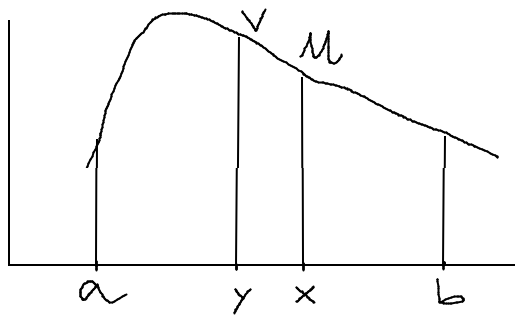
\includegraphics[scale=0.5]{2015T2_3} \end{center}
Resposta correta: (e) [a,x].
\question{Pergunta 4}
\lstinputlisting[language=Python, caption=Programa 2015T2-4 (Python3)]{2015T2_4.py}
A resposta correta é $27.18000$.

\question{Pergunta 5}
\begin{alignat*}{2}
	\frac{d^2y}{dx^2}-A\frac{dy}{dx}+By=0 \iff
	\begin{cases}
		z = \dfrac{dy}{dx}\\
		\dfrac{dz}{dx}=A\,z-B\,y
	\end{cases}
\end{alignat*}
\lstinputlisting[language=Python, caption=Programa 2015T2-5 (Python3)]{2015T2_5.py}

\end{document}
